%
% c06-hyperbolisch.tex
%
% (c) 2008 Prof Dr Andreas Mueller
% $Id: c06-hyperbolisch.tex,v 1.3 2008/10/31 08:04:16 afm Exp $
%
\chapter{Hyperbolische Differentialgleichungen\label{chapter-hyperbolisch}}
\index{Differentialgleichung!partielle!hyperbolische}
\index{Wellengleichung}
\lhead{Hyperbolische PDGL}
\rhead{}
In diesem Kapitel wird als prominentes Beispiel einer hyperbolischen
Differentialgleichung die Wellengleichung diskutiert.
Wie im parabolischen Fall hat die Zeitkoordinate eine spezielle Bedeutung,
auch die Wellengleichung ist eine ``Zeitentwicklungsgleichung'', allerdings
zweiter Ordnung. Während sich eine Änderung der Anfangs- oder Randbedingung
bei einem elliptischen Problem sofort überall auf die Lösung auswirkt,
breiten sich solche Änderungen bei der Wellengleichung mit endlicher
Geschwindigkeit aus. Zu jedem Punkt gibt es also Punkte, auf die sich eine
Wertänderung auswirken kann, und andere, die davon nichts mitbekommen.
Die Grenzflächen zwischen diesen Bereichen sind eine wichtige Grundlage
für das Verständnis der Lösungen.

Zunächst werden daher die Lösungen 
am eindimensionalen Fall bestimmt und die in beide Richtungen laufenden 
Wellenlösungen demonstriert. Diese geben Anlass zu einer Untersuchung,
zu welcher Art von Anfangsbedingung die Wellengleichung überhaupt
lösbar ist. Dies führt uns dann auf den Begriff der Charakteristiken.

\section{Separation}
Oft wird die Wellengleichung auf ein Gebiet der Form
$\Omega = G\times(0,\infty)$ angewandt, also ein 
festes Raumgebiet $G$.
Eine Pauke ändert zum Beispiel die Form des Felles während des
Spielens nicht. In diesen Fällen ist ein Separationsansatz möglich.
Die hyperbolische partielle Differentialgleichung 
\[
\frac1{a^2}\frac{\partial^2 u}{\partial t^2}=\Delta u
\]
kann mit dem Ansatz $u(x,t)=\varphi(x)\cdot T(t)$ in zwei
Differentialgleichungen zerlegt werden:
\begin{gather*}
\begin{aligned}
\frac1{a^2}T''(t)\varphi(x)&=T(t)\Delta \varphi(x)\\
\frac1{a^2}\frac{T''(t)}{T(t)}&=\frac{\Delta\varphi(x)}{\varphi(x)}=\lambda\\
\end{aligned}
\\
\Rightarrow\qquad
T''(t)=\lambda a^2T(t)\qquad\text{und}\qquad\Delta \varphi=\lambda\varphi.
\end{gather*}
Die Differentialgleichung für $T$ ist eine Schwingungsdifferentialgleichung
und stellt damit bezüglich Existenz und Eindeutigkeit der Lösung
kein grosses Problem dar. Wenn $T(0)$ und $T'(0)$ bekannt sind, dann
können wir die Lösung für beliebiges $t$ angeben.

Die zweite Gleichung $\Delta \varphi-\lambda\varphi=0$ ist eine
elliptische partielle Differentialgleichung, über welche wir
in Kapitel~\ref{chapter-elliptisch} einiges an Theorie entwickelt haben.
Zum Beispiel wurde dort gesagt, dass elliptische Probleme auf
zusammenhängenden und beschränkten Gebieten eine eindeutige
Lösung haben, wenn man die Randwerte entlang des gesamten Randes
kennt.

Wir können daraus schliessen, dass das hyperbolische Problem eine
Lösung hat, wenn wir $u(x,0)$ und $\partial_tu(x,0)$ für
$x\in G$ kennen, und ausserdem die Werte $u(x,t)$ für $x\in\partial G$.
Dies passt zu der am Paukenfell gewonnenen Intuition: dessen Schwingung
ist bekannt, wenn Anfangsauslenkung und -geschwindigkeit bekannt sind,
und ausserdem die Randwerte des Felles während der ganzen Zeit
bekannt sind.

Dieses Verfahren versagt aber in Fällen, wo sich das Gebiet verändert,
zum Beispiel bei der Expansion eines Gases.
Die langsame Expansion zum Beispiel in einer Posaune, deren ``Gebiet''
sich ja während des Spielens dauernd verändert, scheint dabei kein
Problem zu sein, jedenfalls kann ein Posaunist auch schwierige Passagen
ohne Studium der Wellengleichung meistern.
Was passiert aber, wenn der
Kolben, der eine Expansionsgefäss verschliesst, mit einer Geschwindigkeit
grösser als die Schallgeschwindigkeit bewegt wird? 

\section{Wellengleichung in einer Dimension}
\rhead{Eindimensionale Wellengleichung}
Die Wellengleichung in der Ebene ist
\[
\partial_t^2u-a^2\partial_x^2u=0,
\]
welche wir auf dem Gebiet
\[
\Omega = \{(x,t) \,|\, t > 0\}
\]
lösen möchten.
$a$ hat die Dimension einer Geschwindigkeit, $a$ ist die
Ausbreitungsgeschwindigkeit der Wellen entlang der $x$-Achse.

\subsection{Konstante Geschwindigkeit}
Wir nehmen an, dass $a$ eine Konstante ist. Dann lässt sich die Gleichung
auch als
\begin{align*}
(\partial_t -a\partial_x)(\partial_t+a\partial_x)u&=0
\\
\text{oder}&
\\
(\partial_t +a\partial_x)(\partial_t-a\partial_x)u&=0
\end{align*}
schreiben.
Offenbar sind Lösungen der folgenden partiellen Differentialgleichungen
erster Ordnung
\begin{align}
\partial_t u-a\partial_x u&=0
\label{wellelinks}
\\
\partial_t u+a\partial_x u&=0
\label{wellerechts}
\end{align}
automatisch auch Lösungen der Wellengleichung.

\subsection{Lösung der partiellen Differentialgleichung erster Ordnung}
Wir möchten die Wellengleichung für eine Anfangsbedingung der Art
\begin{equation}
u(x,t)=u_0(x),\qquad x\in\mathbb R
\label{welleanfang}
\end{equation}
lösen, und suchen daher zunächst Lösungen der beiden
PDGL erster Ordnung (\ref{wellelinks}) und (\ref{wellerechts})
mit genau derselben Anfangsbedingung.

Beide Differentialgleichungen sind quasilineare Differentialgleichungen
erster Ordnung, das Verfahren aus Kapitel~\ref{chapter-geometrie}
liefert dafür eine Lösung. Wir haben dazu zunächst die Lösung der
Gleichung der Charakteristiken zu finden. Diese lautet
\begin{align*}
\frac{dx}{ds}&=-a
\\
\frac{dt}{ds}&=1
\\
\frac{du}{ds}&=0
\end{align*}
Die dritte Gleichung sagt, dass $u$ nicht von $s$ abhängt. Die
zweite Gleichung sagt, dass bis auf eine additive Konstante $s$
und $t$ übereinstimmen, wir können also ohne weiteres $t=s$
wählen. Damit bleibt nur noch die erste Gleichung, welche ebenfalls
einfach zu lösen ist, wir erhalten als Lösung
\begin{equation}
\begin{aligned}
x(s)&=-as+x_0\\
t(s)&=s\\
z(s)&=z_0
\end{aligned}
\label{hyperbolisch:quasi1}
\end{equation}

Der zweite Parameter in der Lösung des Cauchy-Problems ist der
Parameter entlang der Anfangskurve, in unserem Fall ist dies $x_0$,
denn die Anfangskurve wird durch die Werte entlang der $x$-Achse
gegeben. Wir haben also genauer die Gleichungen
\begin{equation}
\begin{aligned}
x(s,x_0)&=-as+x_0\\
t(s,x_0)&=s\\
z(s,x_0)&=u_0(x_0)
\end{aligned}
\label{hyperbolisch:quasi2}
\end{equation}

Der zweite Schritt des Lösungsverfahrens von Kapitel~\ref{chapter-geometrie}
besagt, dass die Variablen $s$ und $x_0$ aus den Gleichungen
(\ref{hyperbolisch:quasi2})
\begin{equation}
u(x(s,x_0), t(s,x_0))=z(s,x_0)
\label{hyperbolisch:quasi3}
\end{equation}
zu eliminieren seien.
Aber aus der zweiten Gleichung 
(\ref{hyperbolisch:quasi2})
folgt $s=t$, und aus
ersten Gleichung von
$x_0=at+x$. Setzt man dies zusammen mit der dritten Gleichung von
(\ref{hyperbolisch:quasi2}) in 
(\ref{hyperbolisch:quasi3}) ein, erhält man
\[
u(x, t)=u_0(x_0)=u_0(at+x).
\]
Als Funktion von $x$ ist
$u(x,t)$ als eine um $at$ nach links verschobene Kopie von $u_0$.
Die Lösung von (\ref{wellelinks})
ist also eine mit Geschwindigkeit $a$ nach links
laufende Welle.

Analog liefert die Gleichung (\ref{wellerechts}) eine mit Geschwindigkeit
$a$ nach rechts laufende Kopie von $u_0$. Da die Wellengleichung linear ist,
ist auch jede Linearkombination dieser beiden Lösungen eine Lösung der
Differentialgleichung. Sind $u_+(x)$ und $u_-(x)$ zwei beliebige Funktionen
derart, dass $u_+(x)+u_-(x)=u_0(x)$, dann ist
\begin{equation}
u(x,t)=u_+(x+at)+u_-(x-at)
\label{dalembertloesung}
\end{equation}
eine Lösung der Wellengleichung mit der Anfangsbedingung (\ref{welleanfang}).

\subsection{Anfangsgeschwindigkeit}
Die Lösung der Wellengleichung ist aber erst durch eine weitere
Anfangsbedingung der Form
\begin{equation}
\partial_tu(x,0)=v_0(x)\label{welleanfangdt}
\end{equation}
vollständig bestimmt.
Wenn sich die Lösung in der Form (\ref{dalembertloesung}) schreiben lassen
soll, muss gelten
\begin{align*}
u_+(x)+u_-(x)&=u_0(x)\\
au_+'(x)-au_-'(x)&=v_0(x)
\end{align*}
Ist $V_0$ eine Stammfunktion von $\frac1av_0$, also $V_0'=\frac1av_0$,
dann folgt aus der zweiten Gleichung, dass 
\[
u_+(x)-u_-(x)=V_0(x)+c.
\]
Diese Gleichungen kann man nach $u_+$ und $u_-$ auflösen:
\begin{align*}
u_+(x)&=\frac12(u_0(x)+V_0(x)+c)\\
u_-(x)&=\frac12(u_0(x)-V_0(x)-c)
\end{align*}
und damit
\begin{align}
u(x,t)
&=
\frac12\bigl(u_0(x+at)+V_0(x+at)+c\bigr)+\frac12\bigl(u_0(x-at)-V_0(x-at)-c\bigr)
\notag
\\
&=
\frac12\bigl(u_0(x+at)+V_0(x+at)\bigr)+\frac12\bigl(u_0(x-at)-V_0(x-at)\bigr)
\label{hyperbolisch:dalembert}
\end{align}
Die Lösung (\ref{hyperbolisch:dalembert})
heisst die d'Alembert-Lösung der Wellengleichung.
\index{d'Alembert}
\index{d'Alembert-L\ösung}

Natürlich sind die einzelnen Summanden Lösungen der Wellengleichung, aber auch
die Anfangsbedingungen sind so erfüllt:
\begin{align*}
u(x,0)&=u_0(x)\\
\partial_tu(x,0)&=\frac12\bigl(au_0'(x+at)+v_0(x)-au_0'(x)+v_0(x)\bigr) =v_0(x)
\end{align*}
Somit lässt sich die Wellengleichung in der Ebene einfach durch Finden einer
Stammfunktion für eine Funktion entlang der $x$-Achse konstruieren.
Das anfangs des Abschnittes
gestellte Problem entspricht dem Fall $v_0(x)=0$.

\section{Das Cauchy-Problem in höheren Dimensionen}
\rhead{Das Cauchy-Problem}
Im letzten Abschnitt haben wir Anfangswerte auf der Geraden $t=0$
vorgegeben, damit waren auch gleichzeitig die Ableitungen 
$\partial_x u(0,x)$ festgelegt. Ausserdem hatten wir mit der Funktion $v_0$
die Ableitungen $\partial_t u(0,x)$ vorgegeben.
Der Graph der Lösungsfunktion ist ein Fläche, eine sogenante
Integralfläche der Differentialgleichung. Die Anfangsbedingung
definiert eine Kurve $x\mapsto(x,0,u_0(x))$, die Integralfläche muss
durch diese Kurve gehen.
Durch die zwei Ableitungen ist zudem in jedem Punkt der Kurve
eine Tangentialebene an die Integralfläche vorgegeben.

Wie das Beispiel zeigt, ist die Lösungsfläche durch Vorgabe einer Kurve und
und der Tangentialebenen in jedem Punkt der Kurve bestimmt ist.
Etwas allgemeiner besteht das Cauchy-Problem darin, eine Integralfläche
zu finden, die durch eine beliebige Kurve geht, und ausserdem in jedem Punkt
der Kurve eine bestimmte Tangentialebene hat. Diese Vorgaben nennt man
einen ``Streifen'' (Abbildung~\ref{skript:streifen}).
Eine partielle Differentialgleichung für eine Funktion $u(t,x,y)$
von drei Variablen kann zum Beispiel dadurch festgelegen werden,
dass man Funktionswerte $u(t,x,y)=u_0(x,y)$ zur Zeit $t=0$ festlegt.
Dadurch sind auch die Ableitungen $\partial_x u(0,x,y)=\partial_xu_0(x,y)$
und $\partial_y u(0,x,y)=\partial_y u_0(x,y)$ bestimmt. Die Lösung wird
aber erst eindeutig bestimmt sein, wenn auch die Ableitung in $t$-Richtung
vorgegeben ist, zum Beispiel in der Form $\partial_t(0,x,y)=v_0(x,y)$.

Allgemeiner besteht das Cauchy-Problem darin, eine Lösung zu finden
die entlang einer beliebigen Fläche im $(t,x,y)$-Raum vorgegebene
Werte annimmt. Ausserdem muss die Richtungsableitungen in eine Richtung
senkrecht auf die Fläche (Normalableitung) ebenfalls vorgegebene Werte annehmen.


\section{Charakteristiken}
\rhead{Charakteristiken}
\subsection{Ein unlösbares Cauchy-Problem}
Wir untersuchen jetzt, unter welchen Voraussetzungen sich das Cauchy-Problem
für eine hyperbolische partielle Differentialgleichung eindeutig lösen lässt.
Um besser zu verstehen, was dabei schief gehen kann, betrachten wir die
hyperbolische partielle Differentialgleichung
\[
\partial_x\partial_y u=0,
\]
und geben die Anfangswerte die
\begin{align*}
u(0,y)&=u_0(y)
\\
\partial_xu(0,y)&=v_0(y)
\end{align*}
vor.
Aus der Differentialgleichung schliessen wir, dass $\partial_y u$
nicht von $x$ abhängt. Somit kann auch $u$ nicht von $x$ abhängen,
die Anfangsbedingung für $\partial_xu(0,y)$ ist also redundant,
sie kann nur erfüllt werden, wenn $v_0(y)=0$.
Die Lösung ist $u(x,y)=u_0(y)$.

Da aber auch $\partial_x\partial_yu=\partial_y\partial_xu$, ist auch
$u(x,y)=g(x)$ eine Lösung der Differentialgleichung. Da diese
Lösung nicht von $y$ abhängt, kann auch die Anfangsbedingung $u(0,y)=u_0(y)$
nicht erfüllt werden. Offenbar ist das Cauchy-Problem nicht lösbar, wenn die
Funktionswerte und Ableitungen auf der Geraden $x=0$ vorgegeben werden.
Ursache dafür ist, dass aus der Differentialgleichung nicht alle zweiten
Ableitungen bestimmt werden können. Die zweite partielle Ableitung
nach $\partial_x^2u(0,y)$ ist unbestimmt.

\subsection{Streifen}
Das Cauchy-Problem kann also nur dann lösbar sein, wenn die Funktionswerte
und die ersten partiellen Ableitungen entlang einer Kurve
auch alle zweiten Ableitungen eindeutig bestimmen.
Wir versuchen daher
diejenigen Kurven zu bestimmen, auf denen dies nicht möglich ist.
Wir gehen aus von der Differentialgleichung
\begin{equation}
a\frac{\partial^2 u}{\partial x^2}
+
2b\frac{\partial^2 u}{\partial x\partial y}
+
c\frac{\partial^2 u}{\partial y^2}
+
d\frac{\partial u}{\partial x}
+
e\frac{\partial u}{\partial y}
+
fu
=g,
\label{charequation}
\end{equation}
Da wir vor allem an den zweiten Ableitungen interessiert sind, bringen
wir alle anderen Terme auf die rechte Seite, und kürzen die neue
rechte Seite mit $h$ ab:
\begin{equation}
a\frac{\partial^2 u}{\partial x^2}
+
2b\frac{\partial^2 u}{\partial x\partial y}
+
c\frac{\partial^2 u}{\partial y^2}
=
g
-
d\frac{\partial u}{\partial x}
+
e\frac{\partial u}{\partial y}
+
fu
=h.
\notag
\end{equation}
Ausserdem betrachten wir eine Kurve
$t\mapsto(x(t),y(t))$.
Entlang der Kurve sind die Anfangswerte
und die partiellen Ableitungen
\begin{equation}
\left.
\begin{aligned}
u(x(t),y(t))&=u(t)\\
\frac{\partial u}{\partial x}(x(t),y(t)) &= p(t)\\
\frac{\partial u}{\partial y}(x(t),y(t)) &= q(t)
\end{aligned}
\qquad
\right\}
\label{charanfangs}
\end{equation}
vorgegeben. Diese Vorgaben nennt man einen {\em Streifen}
(Abbildung~\ref{skript:streifen}).

\begin{figure}
\centering
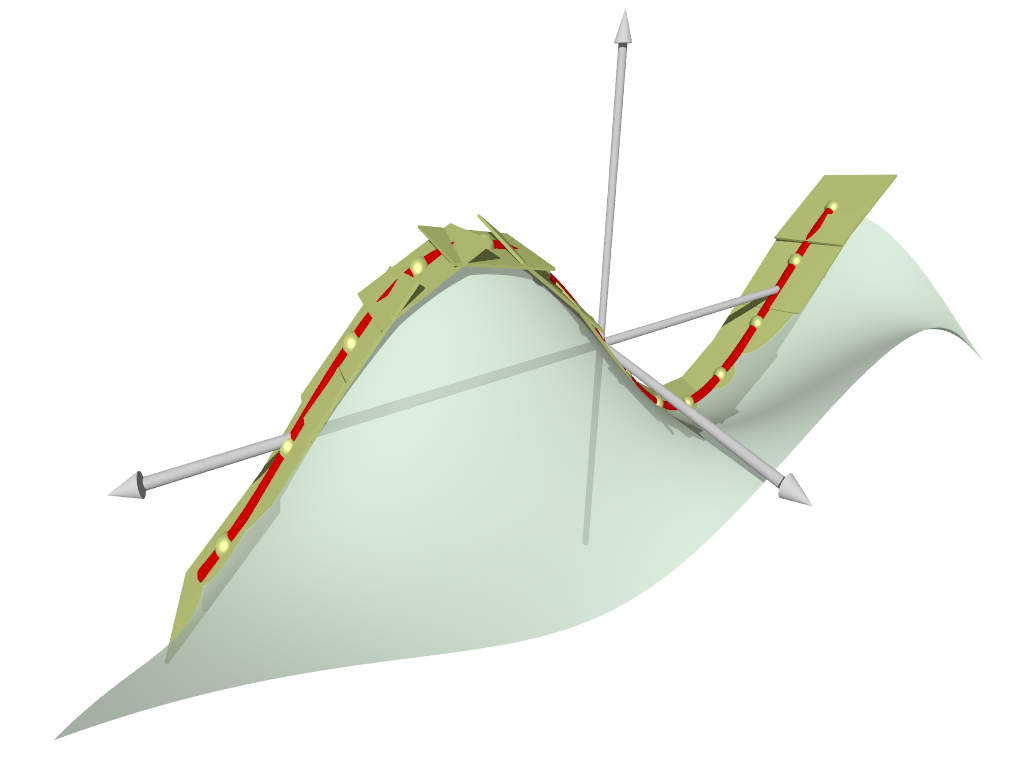
\includegraphics[width=\hsize]{../common/3d/streifen0.png}
\caption{Ein Streifen besteht aus der Vorgabe von Anfangskurve (rot)
und Tangentialbenen.
Die grüne Fläche ist Lösungsfläche der Wellengleichung mit 
dem Streifen als Anfangsbedingung.
\label{skript:streifen}}
\end{figure}

\begin{figure}
\centering
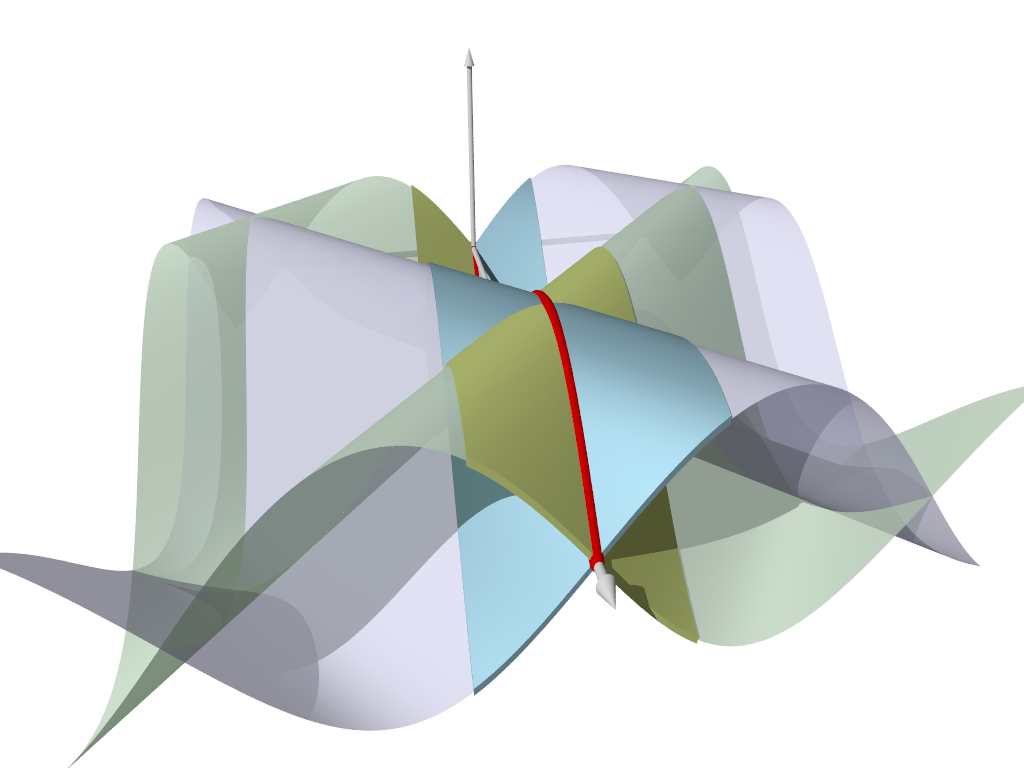
\includegraphics[width=\hsize]{../common/3d/streifen2.png}
\caption{Entlang der gemeinsamen roten Kurve haben die beiden
Lösungsflächen der Wellengleichung verschiedene Tangentialebenen,
also verschiedene Streifen. 
Der Streifen legt die Lösung eindeutig fest.
\label{skript:streifen:eindeutig}}
\end{figure}

\begin{figure}
\centering
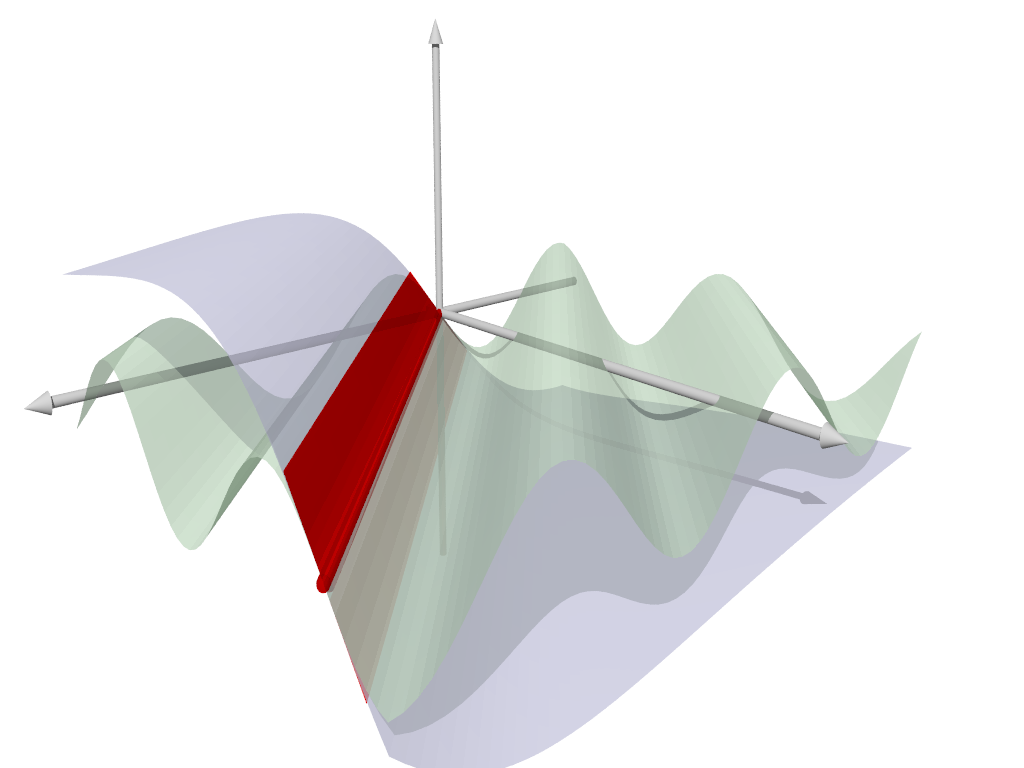
\includegraphics[width=\hsize]{../common/3d/streifen1.png}
\caption{Charakteristiken sind nicht geeignet als Anfangskurven,
weil ein Streifen entlang einer Charakteristik die Lösungsfläche
nicht eindeutig zu bestimmen braucht. Die Abbildung zeigt zwei Lösungen
der Wellengleichung, die sich in dem roten Streifen berühren.
\label{skript:streifen:zweideutig}}
\end{figure}

Die Funktionen $u(t)$, $p(t)$ und $q(t)$ sind nicht ganz willkürlich.
Leitet man nämlich die erste der Gleichungen (\ref{charanfangs}) nach
$t$ ab, findet man
\[
\dot{u}(t)=\frac{d}{dt}u(t)
=
\frac{d}{dt}u(x(t),y(t))
=
\frac{\partial u}{\partial x}(x(t), y(t))\frac{d}{dt}x(t)
+
\frac{\partial u}{\partial y}(x(t), y(t))\frac{d}{dt}y(t).
\]
Die partiellen Ableitungen sind aber ebenfalls in (\ref{charanfangs})
vorgegeben, es muss also die Beziehung
\begin{equation}
\dot{u}(t)= p(t)\dot{x}(t) + q(t)\dot{y}(t)
\label{cauchydatarestriction}
\end{equation}
gelten.

\subsection{Charakteristiken}
Die Vorgabe eines Streifens bestimmt die Lösung einer hyperbolischen
partiellen Differentialgleichung meistens eindeutig.
In Abbildung~\ref{skript:streifen:eindeutig} zeigt zwei verschiedene
Lösungen der Wellengleichung, die entlang der $t$-Achse zwar die
gleiche Anfangskurve, aber verschiedene Tangentialebenen und damit
verschiedene Streifen haben.

Leitet man die letzten zwei Gleichungen von (\ref{charanfangs}) nach $t$ ab,
erhält man
\[
\begin{linsys}{3}
\dot p(t)
&=&
\partial_x\partial_xu(x(t),y(t))\,\dot x(t)
&+&
\partial_x\partial_yu(x(t),y(t))\,\dot y(t)
& &
\\
\dot q(t)
&=&
& &
\partial_x\partial_yu(x(t),y(t))\,\dot x(t)
&+&
\partial_y\partial_yu(x(t),y(t))\,\dot y(t)
\end{linsys}
\]
Zusammen mit der Differentialgleichung haben wir also die folgenden
drei Gleichungen für die rot hervorgehobenen zweiten partiellen Ableitungen:
\[
\begin{linsys}{4}
a{\color{red}\displaystyle\frac{\partial^2 u}{\partial x^2}}
&+&
2b{\color{red}\displaystyle\frac{\partial^2 u}{\partial x\partial y}}
&+&
c{\color{red}\displaystyle\frac{\partial^2 u}{\partial y^2}}
&=&
h(t)
&=&
g-dp(t)-eq(t)-fu\\
\dot x(t)
{\color{red}\displaystyle\frac{\partial^2 u}{\partial x^2}}
&+&
\dot y(t)
{\color{red}\displaystyle\frac{\partial^2 u}{\partial x\partial y}}
& &
&=&
\dot p(t)
& &
\\
& &
\dot x(t)
{\color{red}\displaystyle\frac{\partial^2 u}{\partial x\partial y}}
&+&
\dot y(t)
{\color{red}\displaystyle\frac{\partial^2 u}{\partial y^2}}
&=&
\dot q(t)
& &
\end{linsys}
\]
Dieses lineare Gleichungssystem für die zweiten partiellen Ableitungen
hat die Koeffizientenmatrix
\[
\begin{pmatrix}
a&2b&c\\
\dot x(t)&\dot y(t)&0\\
0&\dot x(t)&\dot y(t)
\end{pmatrix}.
\]
Es ist genau dann nicht oder nicht eindeutig lösbar, wenn die Determinante
verschwindet
\begin{align*}
0&=\left|\begin{matrix}
a&2b&c\\
\dot x(t)&\dot y(t)&0\\
0&\dot x(t)&\dot y(t)
\end{matrix}\right|
\\
&=a\dot y(t)^2-2b\dot x(t)\dot y(t)+c\dot x(t)^2
\end{align*}

\begin{definition}
Die Charakterisitiken einer Differentialgleichung der Form (\ref{charequation})
sind die Kurven $t\mapsto(x(t),y(t))$, für die die Anfangswerte (\ref{charanfangs})
die zweiten partiellen Ableitungen nicht eindeutig bestimmen.
\end{definition}

\begin{satz}
\label{charakteristikendgl}
Die Charakteristiken einer partiellen Differentialgleichung (\ref{charequation})
erfüllen  die Differentialgleichung
\[
a\dot y(t)^2-2b\dot x(t)\dot y(t)+c\dot x(t)^2=0.
\]
\end{satz}

\subsection{Charakteristische Streifen}
Wir wählen jetzt eine Charakteristik $t\mapsto(x(t),y(t))$.
Uns interessiert nur der Fall, in dem es unendlich viele
Lösungen für die zweiten Ableitungen gibt. Dieser tritt dann
ein, wenn auch die Determinanten
\[
\left|
\begin{matrix}
h&2b&c\\
\dot p(t)&\dot y(t)&0\\
\dot q(t)&\dot x(t)&\dot y(t)
\end{matrix}
\right|
,
\quad
\left|
\begin{matrix}
a&h&c\\
\dot x(t)&\dot p(t)&0\\
0&\dot q(t)&\dot y(t)
\end{matrix}
\right|
,
\quad
\left|
\begin{matrix}
a&2b&h\\
\dot x(t)&\dot y(t)&\dot p(t)\\
0&\dot x(t)&\dot q(t)
\end{matrix}
\right|
\]
verschwinden, wobei $h=g-dp(t)-eq(t)-fu(x(t),y(t))$.
Es genügt dabei, eine einzige Determinante zu wählen,
wir wählen die zweite:
\begin{align*}
a\dot p(t)\dot y(t)-h\dot x(t)\dot y(t)+c\dot x(t)\dot q(t)&=0
\end{align*}
Zusammen mit der Bedingung~(\ref{cauchydatarestriction})
%\[
%\dot u=p(t)\dot x(t)+q(t)\dot y(t)
%\]
haben wir jetzt drei Gleichungen, welche die Grössen 
$x$, $y$, $u$, $p$ und $q$ erfüllen müssen, damit die zweiten
Ableitungen auf unendlich viele Arten bestimmt sind.

\begin{definition}
Ein Streifen entlang einer Charakteristik, der zusätzlich die
Bedingung 
\[
a\dot p(t)\dot y(t)-h\dot x(t)\dot y(t)+c\dot x(t)\dot q(t)=0
\]
erfüllt, heisst ein {\em charakteristischer Streifen}.
\end{definition}

Es ist also möglich, dass sich Integralflächen einer Differentialgleichung
in einer Kurve schneiden, dort sogar berühren, aber trotzdem verschieden
sind. Notwendigerweise bilden die Tangentialebenen
entlang der Schnittkurve einen charakteristischen Streifen.

\begin{satz}
\label{skript:satz:charakteristiken}
Berühren sich zwei verschiedene Integralflächen entlang einer
Kurve, dann stellen diese Kurve zusammen mit den zugehörigen Tangentialebenen
einen charakteristischen Streifen dar.
\end{satz}

Abbildung~\ref{skript:streifen:zweideutig} zeigt zwei Lösungen der
Wellengleichung, die sich entlang einer Charakteristik berühren.
Nach Satz~\ref{skript:satz:charakteristiken} ist der rote Streifen ein
charakteritischer Streifen.

\begin{proof}[Beweis]
Offenbar gibt es mindestens zwei Lösungen der Differentialgleichung
durch die gegebene Kurve, die ausserdem die gleichen Tangentialebenen
haben. Die Kurve und die Tangentialebenen bestimmen die Lösung nicht
eindeutig, sie bilden also einen charakteristischen Streifen.
\end{proof}

\subsection{Beispiele}
\subsubsection{Wellengleichung}
Die Charakteristiken der Wellengleichung
\begin{equation}
\partial_t^2u-a^2\partial_x^2u=0
\label{hyperbolisch:wellengleichung}
\end{equation}
sind Kurven $s\mapsto(t(s),x(s))$, die die Gleichung
\begin{align*}
\left(
\frac{dx(s)}{ds}\right)^2-a^2\left(\frac{dt(s)}{ds}\right)^2&=0
\\
\frac{dx(s)}{ds}
&=
\pm a\frac{dt(s)}{ds}
\\
\Rightarrow
\frac{dx}{dt}=\pm a
\end{align*}
erfüllen. Dies sind Geraden mit der Steigung $\pm a$.
\begin{figure}
\begin{center}
\includegraphics[width=0.8\hsize]{../common/images/char-2.pdf}
\end{center}
\caption{Charakteristiken der
Wellengleichung~(\ref{hyperbolisch:wellengleichung})
\label{hyp:wellen}}
\end{figure}
Abbildung~\ref{hyp:wellen} zeigt die Charakteristiken.

\subsubsection{Die Gleichung $\partial_x\partial_yu=0$} Die Bedingung für die
Charakteristiken lautet in diesem Fall
\[
-\dot x(t)\dot y(t)=0
\]
Eine der Ableitungen muss also verschwinden, was nur für Kurven
möglich ist, die parallel zur $x$- oder $y$-Achse verlaufen.
Die Abbildung \ref{hyp:dxdy} zeigt die Charakteristiken.
\begin{figure}
\begin{center}
\includegraphics[width=0.8\hsize]{../common/images/char-3.pdf}
\end{center}
\caption{Charakteristiken der hyperbolischen
partiellen Differentialgleichung
$\partial_x\partial_yu=0$.
\label{hyp:dxdy}}
\end{figure}

\subsubsection{Gekrümmte Charakteristiken}
Die partielle Differentialgleichung
\begin{equation}
\partial_t^2u-x^2\partial_x^2u=0
\label{hyperbolisch:gekruemmt}
\end{equation}
ist für $x\ne 0$ hyperbolisch.
Ihre Charakteristiken erfüllen die Gleichung
\begin{align*}
x'(s)^2-x^2t'(s)^2&=0
\\
xt'&=\pm  x'
\\
\frac{d}{ds}t&=\pm\frac{d}{ds}\log x
\\
t&=\pm\log x+C
\\
x&=x_0e^{\pm t}
\end{align*}
Die Charakteristiken sind also Exponentialkurven. In Abbildung \ref{hyp:exp}
sind die Charakteristiken für das positive Zeichen rot eingezeichnet, die
Charakteristiken für das negative Zeichen dagegen grün.
\begin{figure}
\begin{center}
\includegraphics[width=0.8\hsize]{../common/images/hypexp-1.pdf}
\end{center}
\caption{Charakteristiken der für $x\ne 0$ hyperbolischen
partiellen Differentialgleichung~(\ref{hyperbolisch:gekruemmt}).
\label{hyp:exp}}
\end{figure}

Diese Gleichung beschreibt die Wellenausbreitung in einem Medium,
in dem die Wellengeschwindigkeit mit grösser werdendem $x$ ebenfalls
zunimmt. Die Exponentialkurven deuten an, wie die Wellenbewegung nach ``aussen''
immer schneller wird.

\subsection{Charakteristiken für elliptische und parabolische PDGL}
Die oben entwickelte Theorie der Charakteristiken kann selbstverständlich
auch auf elliptische und hyperbolische PDGL angewendet werden.
Im elliptischen Fall hat die Differentialgleichung der Charakteristiken
\[
a\dot y(t)^2-2b\dot x(t)\dot y(t)+c\dot x(t)^2=0
\]
gar keine Lösung, da der Ausdruck nur dann verschwindet, wenn $\dot x(t)=0$
und $\dot y(t)=0$.

Für parabolische PDGL wird der Ausdruck bei Wahl eines geeigneten
Koordinatensystems zu
\[
-\kappa t'(s)^2=0
\]
dies ist nur möglich, wenn $t$ konstant ist. Die Charakteristiken
sind in diesem Falle also Geraden parallel zur $x$-Achse.
Tatsächlich ist es mit der Differentialgleichung und
den Anfangsbedingungen alleine nicht
möglich, die zweite Ableitung nach $t$ entlang einer solchen Geraden
zu bestimmen.

\subsection{Einige interessante Sätze}

\begin{satz}Jede Integralfläche kann mit einer Schar
charakteristischer Streifen bedeckt werden.
\end{satz}

\begin{proof}[Beweis]
Sei $u$ eine Lösung der Differentialgleichung, die die Integralfläche beschreibt.
Die Differentialgleichung von Satz \ref{charakteristikendgl}
beschreibt in jedem Punkt des Definitionsbereichs zwei Kurven $t\mapsto(x(t),y(t))$,
offenbar kann man den Definitionsbereich mit einer Schar solcher Kurven
überdecken.
Setzen wir diese Kurven in $u(x,y)$, $\partial_xu(x,y)$
und $\partial_yu(x,y)$ ein, erhalten wir eine Schar von charakteristischen
Streifen.
\end{proof}

\begin{satz}Überdeckt eine Schar charakteristischer Streifen
eine Fläche $S$, gegeben durch eine Funktion $u(x,y)$, und hat
diese Funktion stetige Ableitungen bis zur zweiten Ordnung,
dann ist $u$ eine Lösung der Differentialgleichung.
\end{satz}

\begin{proof}[Beweis]
Die charakteristischen Streifen erfüllen die Gleichungen
\begin{equation}
\begin{gathered}
a\dot y(t)^2-2b\dot x(t)\dot y(t)+c\dot x(t)^2=0,
\\
a\dot p(t)\dot y(t)-h\dot x(t)\dot y(t)+c\dot x(t)\dot q(t)=0,
\\
\dot u(t)=p(t)\dot x(t)+q(t)\dot y(t).
\end{gathered}
\label{alle}
\end{equation}
Nennen wir die zweiten Ableitungen von $u$ entlang einer Charakteristik
\begin{align*}
R&=\partial_x^2u(x(t),y(t)),
\\
S&=\partial_x\partial_yu(x(t),y(t)),
\\
T&=\partial_y^2u(x(t),y(t)),
\end{align*}
können wir schreiben
\begin{align*}
\dot p(t)&=R(t)\dot x(t)+S(t)\dot y(t)\qquad\text{und}\\
\dot q(t)&=S(t)\dot x(t)+T(t)\dot y(t)
\end{align*}
Setzen wir dies in die zweite Gleichung von (\ref{alle}) ein, erhalten wir
\begin{align*}
a(R\dot x+S\dot y)\dot y-h\dot x\dot y+c\dot x(S\dot x+T\dot y)&=0
\\
\Rightarrow \qquad(aR-h+cT)\dot x\dot y+aS\dot y^2 +cS \dot x^2&=0.
\end{align*}
Multiplizieren wir die erste Gleichung von (\ref{alle}) mit $S$ und subtrahieren
sie, erhalten wir
\[
(aR+2bS+cT-h)\dot x\dot y=0.
\]
Ausgeschrieben ist der Klammerfaktor
\[
a\partial_x^2u+2b\partial_x\partial_yu+c\partial_y^2u-h=0
\]
Also die ursprüngliche Differentialgleichung.
\end{proof}
Dieser Satz besagt, dass man die hyperbolische Differentialgleichung dadurch
lösen kann, dass man charakteristische Streifen sucht. Dazu genügt
es aber, ein System von gewöhnlichen Differentialgleichungen
für die Funktion $x$, $y$, $p$, $q$, $R$, $S$ und $T$
zu lösen.

\section{Ausbreitung von Unstetigkeiten}
\rhead{Unstetigkeiten}
In der Untersuchung der Lösungen der Wellengleichung zu Beginn
dieses Kapitels wurden Lösungen gefunden, welche durch Verschiebung
einer Anfangswertfunktion $u_0$ entlang der 
Charakteristiken, also der Geraden 
$x\pm at=\operatorname{const}$ erhalten werden können. Ist $u_0$
nicht überall differenziertbar, liefert die Formel immer noch eine
stetige Lösung, die jedoch entlang der Charakteristiken nicht
differenzierbar ist.

Nehmen wir an, $u$ sei mit Ausnahme einer Kurve überall zweimal
stetig differenzierbar.
Auf der Kurve selbst sei nur die erste Ableitung stetig.
Die Kurve teilt den Definitionsbereich in zwei
Bereiche, offenbar ist $u$ in jedem dieser Bereiche eine 
Lösung der Differentialgleichung mit den gleichen Anfangswerten
entlang der Kurve und den gleichen Tangentialebenen.
Da die zweiten Ableitungen aber nicht auch übereinstimmen, muss
die Kurve eine Charakteristik sein.



\begin{satz}
Ist eine Funktion $u$ mit Ausnahme einer Kurve zweimal stetig
differenzierbar, und erfüllt sie die Differentialgleichung
ausserhalb der Kurve, dann ist die Kurve eine Charakteristik.
\end{satz}
Unstetigkeiten können sich also nur entlang von Charakteristiken
ausbreiten.
Die Wellengleichung kann auch zur näherungsweisen
Berechnung der Strömung um ein Überschallflugzeug verwendet werden.
Dabei treten Unstetigkeiten als vom Flugzeug erzeugte Schockwellen
auf, und können als Dichteänderungen mit einer
sogenannten Schlierenaufnahme sichtbar gemacht werden
(Abbildung~\ref{ueberschall2d}).

\begin{figure}
\begin{center}
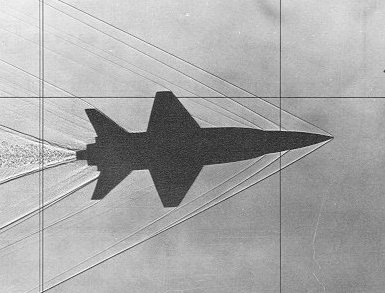
\includegraphics[width=0.8\hsize]{../common/graphics/i-5-1}
\end{center}
\caption{Überschallströmung um ein Überschallflugzeug\label{ueberschall2d}}
\end{figure}

\section{Charakteristiken in höheren Dimensionen}
\rhead{Charakteristiken in höheren Dimensionen}
Wir wollen jetzt die Frage nach den Charakteristiken in höheren Dimensionen
stellen. Um die Diskussion überschaubar zu halten, beschränken wir uns auf
das dreidimensionale Problem. Die gefundenen Schlussfolgerungen 
lassen sich sofort auf beliebig viele Dimensionen verallgemeinern.

\subsection{Problemstellung}
Das Cauchy-Problem für eine partielle Differentialgleichung der
Form
\[
\sum_{i,j=1}^3a_{ij}\partial_i\partial_ju+\sum_{i=1}^3b_i\partial_iu+cu=f
\]
besteht darin, dass auf einer Fläche, die zum Beispiel durch
eine Gleichung
\[
\omega(x_1,x_2,x_3)=0
\]
gegeben werden kann,
die Funktionswerte von $u$ vorgegeben werden, sowie die ersten
Ableitungen in eine Richtung senkrecht auf die Fläche.
Diese Ableitung kann mit Hilfe des Gradienten berechnet werden:
\[
\frac{\partial u}{\partial n}=\operatorname{grad}u\cdot \frac{\operatorname{grad}\omega}{|\operatorname{grad}\omega|}
\]
Die Lösung hängt wieder davon ab, ob die Differentialgleichung
und die Anfangsbedingungen die zweiten Ableitungen von $u$ bereits
eindeutig bestimmen.

\subsection{Ein Spezialfall}
Wir betrachten wieder den Spezialfall, in dem die Anfangswerte auf der
Ebene $x_1=0$ vorgegeben sind, also
\begin{align*}
u(0,x_2,x_3)&=u_0(x_2,x_3),
\\
\partial_1u(0,x_2,x_3)&=h(x_2,x_3)
\end{align*}
Dies entspricht dem Fall $\omega(x_1,x_2,x_3)=x_1$.

Durch die Vorgabe der Anfangswerte in Form der Funktion $u_0$ sind die Ableitungen
$\partial_iu$ für $i=2,3$ ebenfalls festgelegt.
Durch Ableiten der Anfangsbedingungen nach $x_2,\dots,x_3$
sind auch die zweiten Ableitungen 
\[
\partial_i\partial_ju(0,x_2,x_3)\qquad 2\le i\le 3,\;1\le j\le 3
\]
bekannt. Es ist also nur noch $\partial_1^2u$ zu bestimmen.
Die Differentialgleichung kann nach $\partial_1^2u$ aufgelöst
werden, wenn $a_{11}\ne 0$. Dies ist gleichbedeutend damit, dass
\[
a_{11}=\begin{pmatrix}
1&0&\dots&0
\end{pmatrix}
A
\begin{pmatrix}1\\0\\\vdots\\0\end{pmatrix}
=0.
\]

\subsection{Der allgemeine Fall}
Wir betrachten die Funktion $\omega(x_1,x_2,x_3)$ als die erste
Koordinaten eines neuen Koordinatensystems. Die Koordinaten in diesem
neuen System nennen wir $\omega_1,\dots,\omega_3$, sie sind Funktionen
der alten Koordinaten
\[
\omega_1(x_1,x_2,x_3)=\omega(x_1,x_2,x_3)
,\qquad
\omega_2(x_1,x_2,x_3)
,\qquad
\omega_3(x_1,x_2,x_3)
\]
Die Funktion $u$ kann natürlich auch in den neuen Koordinaten geschrieben
werden: $\tilde u(\omega_1,\omega_2,\omega_3)$ hat die Eigenschaft
\[
\tilde u(
\omega_1(x_1,x_2,x_3),
\omega_2(x_1,x_2,x_3),
\omega_3(x_1,x_2,x_3)) = u(x_1,x_2,x_3).
\]
Setzt man dies in die Differentialgleichung ein, ergibt sich
\begin{align*}
\partial_iu
&=
\sum_{k=1}^3
\frac{\partial\tilde u}{\partial \omega_k}
\frac{\partial\omega_k}{\partial x_i}
\\
\partial_i\partial_ju
&=
\sum_{k,l=1}^3
\frac{\partial^2\tilde u}{\partial \omega_k\partial\omega_l}
\frac{\partial\omega_k}{\partial x_i}
\frac{\partial\omega_l}{\partial x_j}
\\
\sum_{i,j=1}^3a_{ij}\partial_i\partial_ju
&=
\sum_{i,j,k,l=1}^3a_{ij}
\frac{\partial^2\tilde u}{\partial \omega_k\partial\omega_l}
\frac{\partial\omega_k}{\partial x_i}
\frac{\partial\omega_l}{\partial x_j}
\\
\sum_{i=1}^3b_i\partial_iu
&=
\sum_{i,k=1}^3b_i
\frac{\partial\tilde u}{\partial \omega_k}
\frac{\partial\omega_k}{\partial x_i},
\end{align*}
die Differentialgleichung für $\tilde u$ in den neuen 
Koordinaten lautet also
\[
\sum_{k,l=1}^3a_{ij}
\biggl(
\sum_{i,j=1}^3a_{ij}
\frac{\partial\omega_k}{\partial x_i}
\frac{\partial\omega_l}{\partial x_j}
\biggr)
\frac{\partial^2\tilde u}{\partial \omega_k\partial\omega_l}
+
\sum_{k=1}^3
\biggl(
\sum_{i=1}^3
b_i
\frac{\partial\omega_k}{\partial x_i}
\biggr)
\frac{\partial\tilde u}{\partial \omega_k}
+c\tilde u
=f.
\]
Die neuen Koeffizienten der zweiten Ableitungen sind also
\[
\tilde a_{kl}=
\sum_{i,j=1}^3a_{ij}
\frac{\partial\omega_k}{\partial x_i}
\frac{\partial\omega_l}{\partial x_j}
\]
Die Fläche entspricht in den $\omega$-Koordinaten dem Spezialfall $\omega_1=0$,
die zweiten Ableitungen sind also genau dann eindeutig bestimmt, wenn
der Koeffizient $\tilde a_{11}$ nicht verschwindet. Entlang der durch $\omega$
definierten Fläche sind also genau dann die zweiten Ableitungen nicht eindeutig
bestimmt, wenn 
\[
\sum_{i,j=1}^3
a_{ij}
\frac{\partial\omega}{\partial x_i}
\frac{\partial\omega}{\partial x_j}
=
\operatorname{grad}\omega
\cdot
A
\operatorname{grad}\omega
=0
\]
Da der Gradient senkrecht auf der Fläche steht, also alle Flächen
problematisch, deren Normalen $\vec n$ die Vektorgleichung
\[
\vec n\cdot A\vec n=0
\]
erfüllen. Diese Vektoren heissen {\em charakteristische Normalen}.

\begin{definition}
Eine durch $\omega(x_1,\dots,x_n)=0$ definierte Fläche heisst
charakteristische Fläche, wenn auf der Fläche
\[
\sum_{i,j=1}^na_{ij}\partial_i\omega\partial_j\omega=0
\]
gilt.
\end{definition}

\subsection{Charakteristische Flächen der Wellengleichung}
\begin{figure}
\begin{center}
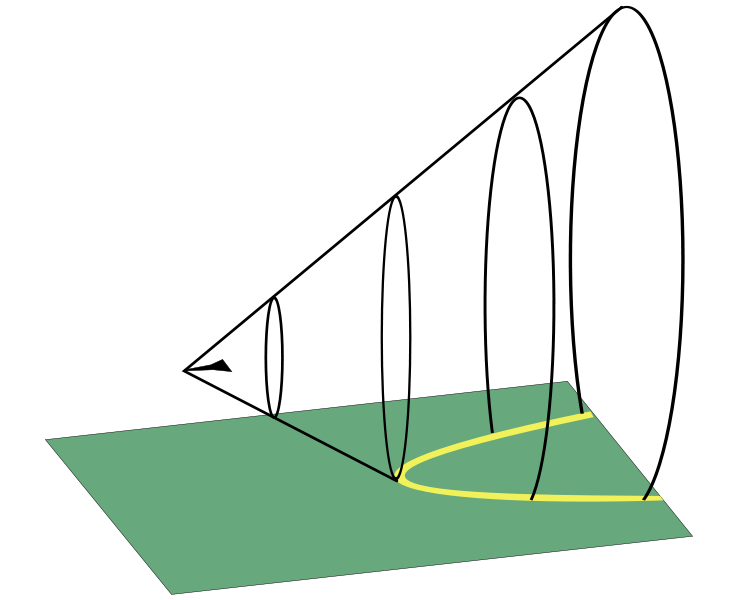
\includegraphics[width=0.8\hsize]{../common/graphics/shock}
\end{center}
\caption{Schockwelle eines Überschallflugzeugs als Beispiel einer
charakteristischen Fläche von $\partial_t^2u-a^2\Delta u=0$.\label{ueberschallkegel}}
\end{figure}
Wir bestimmen die charakteristischen Flächen der
Wellengleichung
\[
\partial_t^2u-a^2\Delta u=0.
\]
Die Koeffizientenmatrix ist
\[
\begin{pmatrix}
1&0&0\\
0&-a^2&0\\
0&0&-a^2
\end{pmatrix},
\]
die charakteristischen Normalen sind also Vektoren $\vec v$, welche die
Gleichung
\[
v_1^2-a^2v_2^2-a^2v_3^2=0
\]
erfüllen. Diese beschreibt einen Doppelkegel, alle Vektoren, welche mit
der $x_1$-Achse einen festen Winkel einschliessen, sind charakteristische
Normalen. Der Winkel $\alpha$ muss der Bedingung
\[
\cos^2\alpha-a^2\sin^2\alpha=0
\]
genügen, also
\[
\tan\alpha=\pm\frac1a.
\]

Die Winkelbedingung ist die einzige Einschränkung an
die charakteristischen Flächen,  entsprechend gibt es eine
grosse Vielfalt:
\begin{enumerate}
\item
Jeder Kegel mit halbem Öffnungswinkel $\frac{\pi}2-\alpha$
und Achse parallel zur $x_1$-Achse ist eine charakteristische Fläche.
Der Kegel schneidet cie $x_2$-$x_3$-Ebene in einem Kreis, dessen Radius mit
grösser werdendem $x_1$ mit der Geschwindigkeit $a$ grösser wird.

Abbildung \ref{ueberschallkegel}
zeigt die Schockwelle eines Überschallflugzeuges. Schockwellen
als Unstetigkeiten müssen sich entlang der charakteristischen Flächen ausbreiten,
also entlang eines Kegels.
\item 
Jede Ebene, die mit der $x_1$-Achse einen Winkel von $\frac\pi2-\alpha$
einschliesst, ist charakteristische Fläche.
Die Ebene schneidet die $x_2$-$x_3$-Ebene in einer Geraden, die sich
mit der Geschwindigkeit $a$ senkrecht zur Geraden fortbewegt.
Diese charakteristische Fläche beschreibt die Fortpflanzung einer
ebenen Welle.
\end{enumerate}


\section{Welche Randwerte beeinflussen die Lösung in einem Punkt?}
\begin{figure}
\centering
\includegraphics{../common/images/kausal-1.pdf}\qquad\qquad%
\includegraphics{../common/images/kausal-2.pdf}
\caption{Randwerte und Punkte des Gebietes, die Einfluss auf einen
Funktionswert der Lösung haben.
Bei einer elliptischen Differentialgleichung $\Delta u=f$
(links)
hängt jeder Funktionswert von jedem Randwert und von jedem Wert der
Funktion $f$ ab.
Die Lösung einer quasilinearen partiellen Differentialgleichung  (rechts)
im Punkt $x$ hängt vom Randwert im Anfangspunkt $x_0$ einer Charaketeristik
ab, die durch $x$ verläuft.
\label{einflussmenge1}}
\end{figure}
\begin{figure}
\centering
\includegraphics{../common/images/kausal-3.pdf}\qquad\qquad%
\includegraphics{../common/images/kausal-4.pdf}
\caption{Randwerte und Punkte des Gebietes, die Einfluss auf einen
Funktionswert der Lösung haben.
Die Lösung einer parabolischen partiellen Differentialgleichung
zur Zeit $t$ hängt von allen Werten $t'<t$ ab.
Bei einer hyperbolischen partiellen Differentialgleichung beinflussen 
nur die Funktionswerte innerhalb eines vom Punkt $x$ ausgehenden Kegels
von Charakteristiken den Wert der Lösung im Punkt $x$.
\label{einflussmenge2}}
\end{figure}
Mit der entwickelten Theorie ist es jetzt möglich, einen Antwort auf die
Frage zu geben, welche Punkte auf dem Rand oder auch im Inneren des Gebietes
einen Einfluss auf die Lösung einer partiellen Differentialgleichung
der Form $Lu=f$ haben.

Im Kapitel~\ref{chapter-elliptisch} haben wir für die Lösung einer
elliptischen partiellen Differentialgleichung eine Formel angegeben,
die $u(x)$ aus allen Randwerten $g$ und der Funktion $f$ in allen 
inneren Punkten berechnet:
\[
u(x)
=
\int_\omega G(x,\xi)f(\xi)\,d\xi
+
\int_{\partial\Omega} \operatorname{grad}_\xi G(x,\xi)g(\xi)\,d\xi.
\]
Eine Änderung von $g$ in irgend einem Punkt des Randes wird im allgemeinen
Die Lösung $u(x)$ verändern, ebenso eine beliebige Änderung von $f$
(Abbildung~\ref{einflussmenge1}, links).

Im Gegensatz dazu wurde im Kapitel~\ref{chapter-geometrie} gezeigt, 
dass die Lösung einer quasilinearen partiellen Differentialgleichung
erster Ordnung im Punkt $x$ nur vom Wert der Anfangsbedingung im Anfangspunkt
derjenigen Charakteristik abhängt, die durch $x$ verläuft
(Abbildung~\ref{einflussmenge1}, rechts).

Die Lösung einer parabolischen partiellen Differentialgleichungen 
kann ebenfalls mit Hilfe einer Greenschen Funktion ausgedrückt werden.
Die Formel~(\ref{green-parabolisch}) zeigt, dass die Werte $u(t,x)$
im Allgemeinen von allen Randwerten $g(t',\xi)$ und $f(t',\xi)$
mit $t'<t$ abhängt (Abbildung~\ref{einflussmenge2}, links).

Die Charakteristischen Flächen (Kurven) beantworten die entsprechende
Frage für eine hyperbolische partielle Differentialgleichung.
Die charakteristischen Flächen (Kurven), die durch den Punkte $x$ verlaufen,
definieren einen Kegel.
Der Wert $u(x)$ der Lösung im Punkt $x$ hängt ab von den
Funktionswerten der rechten Seite der Gleichung und den Randwerten
in diesem Kegel
(Abbildung~\ref{einflussmenge2}, rechts).

\section{Zusammenfassung: das Wichtigste in Kürze}
\begin{enumerate}
\item Jede Lösungsfläche einer hyperbolischen partiellen Differentialgleichung
kann mit charakteristischen Streifen überdeckt werden.
\item Unstetigkeiten breiten sich entlang von Charakteristiken aus.
\item Wie bei quasilinearen partiellen Differentialgleichungen erster
Ordnung kann mit Hilfe der Charakteristiken abgeschätzt werden, wo
Randwerte und Ableitungen vorgegeben werden müssen, damit ein hyperbolisches
Problem gut gestellt ist.
\end{enumerate}

